\documentclass[11pt]{article}

%\usepackage[T2A]{fontenc}     % внутренняя T2A кодировка TeX
\usepackage[russian]{babel}   % включение сов
\usepackage[utf8]{inputenc}
\usepackage[margin=0.25in]{geometry}
\pagestyle{empty} % нумерация выкл.
\addtolength{\textheight}{1.75in}
\usepackage[colorlinks]{hyperref}
\usepackage{longtable}
\usepackage{color}
\usepackage{setspace}
\usepackage{multirow}
\usepackage{graphicx}

\usepackage{fontawesome5} % Для различных контактов

% Заголовки по центру:
\usepackage{titlesec}
\titleformat{\section}{\filcenter\normalfont\Large\bfseries}{\thesection.}{0.2em}{}

%\usepackage[dvipsnames]{xcolor} % Изменение цвета фона
\usepackage[most]{tcolorbox}

% Работа с изображениями:
%\usepackage{tikz}

\definecolor{block-blue}{rgb}{0.8, 0.9, 1}
\newtcolorbox{textblock}[2][]{colback=block-blue,
	boxrule=0pt,boxsep=0pt,breakable}

% Изменить заголовок списка литературы
\addto\captionsrussian{\def\refname{Публикации и ресурсы}}

\usepackage{graphicx}
\makeatletter
\bibliographystyle{unsrt}
\renewcommand{\@biblabel}[1]{#1.} 
\makeatother

\renewenvironment{itemize}{
	\begin{list}{\labelitemi}{
			\setlength{\topsep   }{0pt}
			\setlength{\partopsep}{0pt}
			\setlength{\parskip  }{0pt}
			\setlength{\parsep   }{0pt}
			\setlength{\itemsep  }{0pt}
		}
	}{\end{list}}

\begin{document}
	\vspace*{-\baselineskip} % Удаление отсупа
	\noindent
	\begin{tabular}{p{0.19\textwidth} p{0.78\textwidth}}
		{\centering
			\raisebox{-\totalheight}{
				\begin{tikzpicture}
					\clip (0,0) circle (2cm);
					\node[anchor=center] at (0,-0.1) {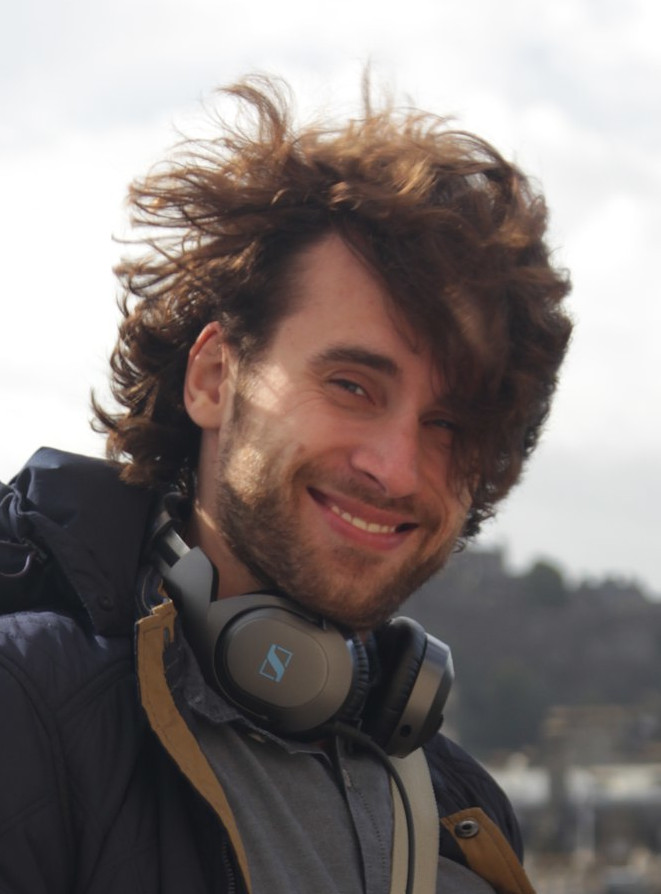
\includegraphics[width=4cm]{ava}};
					%adjust this coordinate to move image
				\end{tikzpicture}
			}
			\href{https://github.com/NikitaShubin/}{{\sffamily{\LARGE{\textbf{\\\faGithub~GitHub}}}}}
		}&
		\raisebox{-\totalheight}{\begin{textblock}
			\noindent {\sffamily{\Huge{\textbf{Никита Шубин}}}}
			5~сентября~1986 | г. Рязань (возможен переезд)\\
			\noindent\faMobile~+7 920 633 94 11 | \href{mailto:shubin.kit@ya.ru}{\faEnvelope~shubin.kit@ya.ru} | \href{https://t.me/kitbrain}{\faTelegram~@kitbrain}
			\vspace{1em}\hrule\vspace{1em}
			\noindent {\textbf{Профиль:}} Team Lead/Data Techlead/Senior Data Scientist (DL, CV).\\ \href{https://disk.yandex.ru/i/ffl8gXNlYxGT8g}{Кандидат технических наук}.
			Решаю задачи технического зрения с 2007~г.
			\vspace{1em}\hrule\vspace{1em}
			
			\noindent\begin{tabular} {llllllll}
				\textbf{Навыки:} & Keras & TensorFlow & PyTorch & Sklearn & CVAT & OpenCV\\
				Photoshop{\textbackslash}Premier & Numpy & Matplotlib & Pandas & YOLO & U-Net & VAEGAN & \\
				3DS Max{\textbackslash}Blender &  FFmpeg & Linux & Docker & \LaTeX & Git & English B1+\\
				
			\end{tabular}
		\end{textblock}}
		%\vspace*{-\baselineskip} % Удаление отсупа после списка
	\end{tabular}
	%\pagecolor{gray}
	%\vspace{0.5em}
		%\section*{Опыт работы:}	
		\noindent {\sffamily{\Large{\textbf{Опыт работы:}}}}
		\vspace{0.9em}\\
		\noindent {\sffamily{\large{\textbf{2023 -- настоящее время: ML Team Lead в \href{https://agrodigit.ru/}{ООО <<ЦПТ <<Агроцифра>>}.}}}}\\
		\begin{tabular} {r|p{0.863\textwidth}}
			Проекты & Автопилот комбайна и силосопровода (автозаполнение кузова).\\
			\noindent{Достижения} & 
			\begin{itemize}
				\item Выстроил конвейер обработки видеоданных для пополнения датасетов и организовал команду разметки.
				\item Разработал ПО, радикально упрощающее процесс разметки данных в \href{https://www.cvat.ai/}{CVAT}, используя предразметку с Segment Anything Model \href{https://segment-anything.com/}{v1} и  \href{https://sam2.metademolab.com/demo}{v2}.
				\item Обучил модели, решающие поставленные задачи.
			\end{itemize}
		\end{tabular}
		\vspace{0.3em}\hrule\vspace{0.1em}\hrule\vspace{0.5em}
		
		\noindent {\sffamily{\large{\textbf{2022 -- 2023: Руководитель ML-направления в ООО <<ЭДС>>.}}}}\\
		\begin{tabular} {r | p{0.863\textwidth}}
			Задачи & Сегментация и детекция объектов на фото и видео (NDA).\\
			Достижения &
			\begin{itemize}
				\item Снизил частоты ложных обнаружений на 70\% и пропусков на 15\% в задаче бинарной сегментации.
				\item Обнаружил и устранил методологическую ошибку, приведшую к утечке данных (data leakage) в датасете и завышению показателей качества на тестовых данных.
				\item Успешно решил проблему объединения, парсинга и балансировки трёх источников данных, представленных в разных форматах.
				\item Выступая в роли Product Owner-а, довёл разработку генератора синтетического датасета с использованием игрового движка \href{https://www.unrealengine.com/en-US/unreal-engine-5}{Unreal Engine 5} до MVP.
			\end{itemize}
			%\vspace*{-\baselineskip} % Удаление отсупа после списка
		\end{tabular}
		\vspace{0.3em}\hrule\vspace{0.1em}\hrule\vspace{0.5em}
		
		\noindent {\sffamily{\large{\textbf{2021 -- 2022: TeamLead видеогруппы машинного обучения в \href{https://www.stream-labs.com/}{Stream Labs}.}}}}\\
		\begin{tabular} {r | p{0.863\textwidth}}
			Задачи & Постановка диагнозов по 1D (ЭКГ), 2D (фото сетчатки глаза) и 3D-данным (КТ лёгких). \\
			Достижения &
			\begin{itemize}
				\item Разработана модель нейронной сети для классификации ЭКГ, которая была интегрирована в систему \href{https://va1235.wixsite.com/tis-tat/edinyj-kardiolog-respubliki-tatarst}{«Единый кардиолог Республики Татарстан»}.
				\item Проект, посвящённый поиску патологий в компьютерной томографии лёгких, доведён до состояния прототипа.
			\end{itemize}
			%\vspace*{-\baselineskip} % Удаление отсупа после списка
		\end{tabular}
		\vspace{0.3em}\hrule\vspace{0.1em}\hrule\vspace{0.5em}
		
		\noindent {\sffamily{\large{\textbf{2020 -- 2021: Программист-исследователь в \href{https://www.spiritdsp.com/company/}{Spirit DSP}.}}}}\\
		\begin{tabular} {r | p{0.863\textwidth}}
			Задачи &
			\begin{itemize}
				\item Разработка видеокодека на основе нейронных сетей.
				\item Замена фона на видео.
			\end{itemize}
			%\vspace*{-\baselineskip} % Удаление отсупа после списка
			\\
			Достижения &
			Предложил и программно реализовал способ кодирования видео, вошедший в PoC.
		\end{tabular}
		\vspace{0.3em}\hrule\vspace{0.1em}\hrule\vspace{0.5em}
		
		\noindent {\sffamily{\large{\textbf{2007 -- 2020: Инженер-программист в \href{http://www.rsreu.ru/}{ФГБОУ ВО <<РГРТУ>>}.}}}}\\
		\begin{tabular} {r | p{0.863\textwidth}}
			Задачи &
			\begin{itemize}
				\item Разработка и исследование алгоритмов и методов обработки изображений и видео.
				\item Написание научных статей и участие в конференциях с докладами.
				\item Написание и проведение лекций и лабораторных работ для студентов ВУЗа.
			\end{itemize}
			%\vspace*{-\baselineskip} % Удаление отсупа после списка
			\\
			Достижения &
			\begin{itemize}
				\item Мои проекты, посвящённые обнаружению линий и границ на изображении, получили поддержку грантов \href{https://www.rfbr.ru/project_search/350568/}{РФФИ}, \href{https://grants.extech.ru/grants/res/winners.php?OZ=9&TZ=K&year=2016}{Гранта Президента} и \href{http://rscf.ru/sites/default/files/docfiles/Winners_0029.pdf}{РНФ};
				\item \href{https://ryazan.bezformata.com/listnews/aspiranti-rgrtu-pobediteli-konkursa/81548415/}{«Молодой ученый года 2020»};
				\item \hyperlink{AutorIDs}{40 публикаций в сборниках трудов конференций и научных журналах};
				\item 2 патента на полезную модель и 1 свидетельство регистрации программы для ЭВМ.
			\end{itemize}
			%\vspace*{-\baselineskip} % Удаление отсупа после списка
		\end{tabular}
	
	\newpage
	
	\noindent {\textbf{Образование:}}\\
	\begin{tabular} {c | c | c}
		2008 -- 2011 & Аспирантура & \href{http://www.rsreu.ru/faculties/faitu/kafedri/aitu}{каф. Автоматики и информационных технологий в управлении.}\\
		2003 -- 2008 & \href{http://www.rsreu.ru/}{ФГБОУ ВО «РГРТУ»} & \href{http://www.rsreu.ru/faculties/faitu/kafedri/aitu}{каф. Автоматики и информационных технологий в управлении.}\\
	\end{tabular}\\

	\noindent{\textbf{Самообразование:}}
	\begin{itemize}
		\item Курс <<\href{https://lab.karpov.courses/certificate/752f8aad-7f6e-40ad-98c2-12efe12bc0b7/}{System Design}>>;
		\item Профессианальная переподготовка по программе «\href{https://disk.yandex.ru/i/H5-s3Lw6j-1wkg}{Data science, нейронные сети, машинное обучение и искусственный интеллект}» (дипломный проект: \href{https://github.com/NikitaShubin/Inpainting}{Inpainting}) и «\href{https://disk.yandex.ru/i/t3yNB56C3nNo5A}{Продвинутый курс}»;
		\item Курс <<\href{https://www.coursera.org/account/accomplishments/certificate/DMUZAUCWBQG4}{Построение выводов по данным}>>;
		\item Курс <<\href{https://www.coursera.org/account/accomplishments/certificate/H8BWKAK4Y96D}{Поиск структуры в данных»}>>;
		\item Курс <<\href{https://www.coursera.org/account/accomplishments/certificate/9GQC5C4UP9YB}{Обучение на размеченных данных}>>;
		\item Курс <<\href{https://www.coursera.org/account/accomplishments/certificate/2AZHZW96L%J2N}{Математика и Python для анализа данных}>>;
		\item Курс <<\href{https://www.coursera.org/account/accomplishments/certificate/6K5Z2UFA5887}{Введение в машинное обучение}>>.
	\end{itemize}
	\vspace{1em}
	\noindent{Appendix}
	\hrule
	\vspace{1em}
	\noindent\hypertarget{AutorIDs}{\textbf{Идентификаторы автора научных публикаций:}}
	\vspace*{-\baselineskip} % Удаление отсупа после списка
	\vspace{0.5em}
	\begin{longtable} {r | l}
		WoS ResearcherID: & \href{https://publons.com/researcher/2345963/nikita-y-shubin/}{\underline{N-5016-2015}}\\
		Scopus AuthorID: & \href{https://www.scopus.com/authid/detail.uri?authorId=56094972000}{\underline{56094972000}}\\
		Orcid: & \href{https://orcid.org/0000-0003-4563-5643}{\underline{0000-0003-4563-5643}}\\
		Google Scholar Citations ID: & \href{https://scholar.google.com/citations?user=auKREHMAAAAJ}{\underline{auKREHMAAAAJ}}
	\end{longtable}
	
\end{document}
